\documentclass[11pt]{article}
\makeatletter\def\input@path{{../}}\makeatother
\usepackage{preamble}
\renewcommand{\chaptername}{Chapter 9: Statistical properties of Bayesian methods}
\graphicspath{{figures/}}

\begin{document}

\solutionstitlepage{9}{Statistical properties of Bayesian methods}{All numbers and figures are reproduced by \texttt{ch09/code/ch09.R} (base R, under one second).}

\tableofcontents
\clearpage

\section*{Answers at a glance}
\addcontentsline{toc}{section}{Answers at a glance}
\begin{center}
\small
\renewcommand{\arraystretch}{1.25}
\begin{tabular}{>{\bfseries\color{navy}}r p{0.82\linewidth}}\toprule
1 & $\mu\mid Y\sim\dist N(Y/2,1)$; $c=0.5$ (equal costs), $c=10/11$ (type I ten times worse); type I error $=1-\Phi(\sqrt2\,\Phi^{-1}(c))$; $c=0.878$ gives 0.05.\\
2 & Run the trial iff $c\{0.8\theta+0.05(1-\theta)\}>1$, i.e.\ $\theta>\frac{1/c-0.05}{0.75}$ (never if $c\le1.25$).\\
3 & $\hat\theta_1$ unbiased, $\hat\theta_2$ biased toward $\frac12$ but less variable; $\hat\theta_2$ wins iff $\theta_0(1-\theta_0)>\frac{n}{12n+4}$ (roughly $0.09<\theta_0<0.91$).\\
4 & Mean $\frac{b+\sum Y_i^2/2}{a+n/2-1}=24.99$, mode $\frac{b+\sum Y_i^2/2}{a+n/2+1}=16.66$; both $\to\sigma^2$.\\
5 & Jeffreys intervals have roughly nominal \emph{average} coverage (0.95--0.96 for $n\ge5$) but fluctuate (0.89--0.99) because $Y$ is discrete.\\
6 & SE $=0.70$; flat prior: $\beta_1\mid\text{data}\approx\dist N(1.8,0.70^2)$, $\Prob(\beta_1>0)=0.995$; sceptical priors shrink it.\\
7 & $n\approx\theta(1-\theta)/0.01^2-3=2{,}397$.\\
8 & $\psi=\eta^2/2$ (normal), $\psi=e^\eta$ (Poisson); MLE $\bar Y$ unbiased; conjugate $\pi(\eta)\propto e^{n_0y_0\eta-n_0\psi(\eta)}$; Bayes estimator $\frac{n_0y_0+n\bar Y}{n_0+n}$, never unbiased for a proper prior.\\\bottomrule
\end{tabular}
\end{center}
\clearpage

% ================================================================= primer
\section*{A five-minute primer on the tools of this chapter}
\addcontentsline{toc}{section}{Primer: the tools of this chapter}

\begin{recall}
\textbf{1. Decision theory.} Choose the action $a$ minimising the \emph{posterior expected loss} $\E[L(\theta,a)\mid\mathbf Y]$. For a test with loss $c_{I}$ for a type I error (rejecting a true $H_0$) and $c_{II}$ for a type II error, reject $H_0$ iff
\[
c_{I}\,\Prob(H_0\mid\mathbf Y)<c_{II}\,\Prob(H_1\mid\mathbf Y)\iff\Prob(H_1\mid\mathbf Y)>\frac{c_I}{c_I+c_{II}}.
\]
Under squared-error loss the Bayes estimator is the posterior mean.

\medskip
\textbf{2. Frequentist properties.} Fix the true parameter $\theta_0$ and imagine repeating the experiment. For an estimator $\hat\theta$: $\text{bias}=\E(\hat\theta)-\theta_0$, and $\text{MSE}=\text{bias}^2+\V(\hat\theta)$. For an interval: coverage $=\Prob(\theta_0\in\text{interval})$.

\medskip
\textbf{3. Asymptotics.} With lots of data the posterior is approximately $\dist N(\hat\theta_{\text{MLE}},\ \text{SE}^2)$ whatever the (smooth, positive) prior --- the Bernstein--von Mises theorem. This lets us do a Bayesian analysis from a reported estimate and standard error.

\medskip
\textbf{4. Exponential families.} $f(y\mid\eta)\propto\exp\{y\eta-\psi(\eta)\}$ has $\E(Y)=\psi'(\eta)$ and $\V(Y)=\psi''(\eta)$; the conjugate prior has the same form in $\eta$.
\end{recall}

\clearpage

% ================================================================= Exercise 1
\exercise{9.1 --- Choosing the rejection threshold}

\begin{problem}{1}
Assume $Y|\mu\sim\dist{Normal}(\mu,2)$ and $\mu\sim\dist{Normal}(0,2)$ (i.e., $n=1$). The objective is to test the null hypothesis $H_0:\mu\le0$ versus the alternative hypothesis that $H_1:\mu>0$. We will reject $H_0$ if $\Prob(H_1|Y)>c$.
\begin{enumerate}[(a)]
\item Compute the posterior of $\mu$.
\item What is the optimal value of $c$ if Type I and Type II errors have the same costs?
\item What is the optimal value of $c$ if a Type I error costs ten times more than a Type II error?
\item Compute the Type I error rate of the test as a function of $c$.
\item How would you pick $c$ to control Type I error at 0.05?
\end{enumerate}
\end{problem}

\begin{restate}
One normal observation, a normal prior, and the rule ``reject if the posterior probability of $\mu>0$ exceeds $c$''. Choose $c$ from costs, then study how often the rule rejects a true null.
\end{restate}

\begin{recall}
Normal--normal update (Chapter 2 primer); decision rule for tests (primer, point 1). Both variances here are 2 (the second argument of $\dist{Normal}$ is the variance).
\end{recall}

\begin{keyidea}
$\Prob(H_1\mid Y)=\Phi(Y/2)$ is increasing in $Y$, so ``$\Prob(H_1\mid Y)>c$'' is the same as ``$Y>$ a cut-off''; the type I error is a normal tail probability at the boundary $\mu=0$.
\end{keyidea}

\solution
\step{(a) Posterior.} Precisions $\frac12+\frac12=1$; mean $\frac{Y/2+0}{1}=\frac Y2$. So $\mu\mid Y\sim\dist{Normal}(Y/2,\ 1)$ and $\Prob(H_1\mid Y)=\Prob(\mu>0\mid Y)=\Phi(Y/2)$.
\step{(b) Equal costs.} $c=\frac{c_I}{c_I+c_{II}}=\frac{1}{2}$: reject when $H_1$ is more probable than $H_0$ (i.e.\ when $Y>0$).
\step{(c) Type I error ten times worse.} $c=\frac{10}{10+1}=\frac{10}{11}=0.909$.
\step{(d) Type I error.}
Reject iff $\Phi(Y/2)>c\iff Y>2\Phi^{-1}(c)$. Under $H_0$ the probability of rejection is largest at the boundary $\mu=0$, where $Y\sim\dist N(0,2)$:
\[
\alpha(c)=\Prob\big(Y>2\Phi^{-1}(c)\mid\mu=0\big)=1-\Phi\Big(\frac{2\Phi^{-1}(c)}{\sqrt2}\Big)=1-\Phi\big(\sqrt2\,\Phi^{-1}(c)\big).
\]
For example $\alpha(0.5)=0.5$ and $\alpha(10/11)=0.030$.
\begin{center}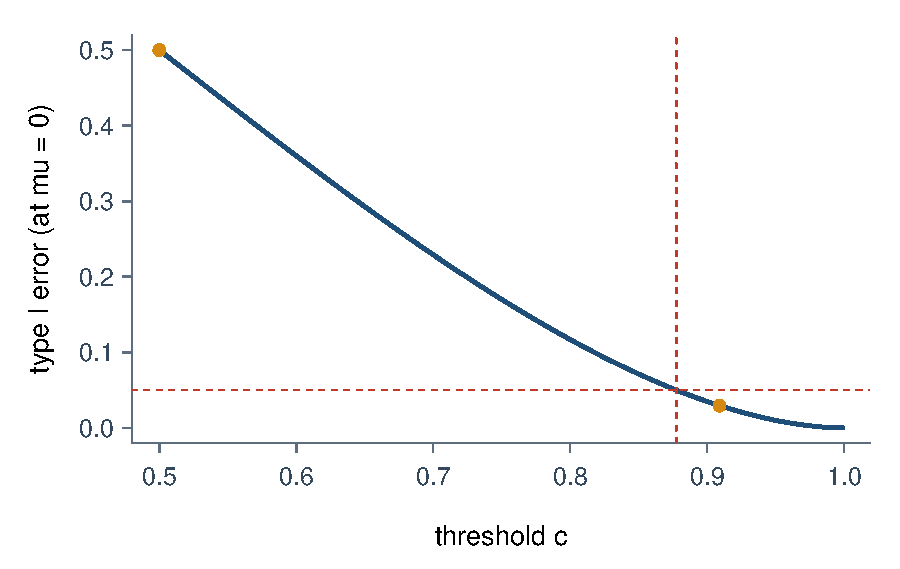
\includegraphics[width=0.62\linewidth]{ex01_type1.pdf}\end{center}
\step{(e) Controlling type I error at 0.05.} Solve $\alpha(c)=0.05$: $\sqrt2\,\Phi^{-1}(c)=1.645\Rightarrow\Phi^{-1}(c)=1.163\Rightarrow c=\Phi(1.163)=\mathbf{0.878}$.

\begin{sanity}
$10^6$ simulated datasets with $\mu=0$ and $c=0.8776$ reject 5.01\% of the time. \checkmark
\end{sanity}

\begin{answer}
(a) $\mu\mid Y\sim\dist N(Y/2,1)$. (b) $c=0.5$. (c) $c=10/11\approx0.909$. (d) $\alpha(c)=1-\Phi(\sqrt2\,\Phi^{-1}(c))$ (worst case $\mu=0$). (e) $c=\Phi(1.645/\sqrt2)=0.878$.
\end{answer}

\begin{takeaway}
A Bayesian threshold can be chosen from costs (decision theory) or calibrated to a frequentist error rate; here a 10:1 cost ratio already gives a type I error of only 3\%.
\end{takeaway}

% ================================================================= Exercise 2
\exercise{9.2 --- Should the company run the confirmatory trial?}

\begin{problem}{2}
Given data from a small pilot study, your current posterior probability that the new drug your company has developed is more effective than the current treatment is $\theta\in[0,1]$. Your company is considering to run a large clinical trial to confirm that your drug is indeed preferred. If you run the trial it will cost $X$. \emph{If in fact your drug is better, then the probability that you will confirm this in the trial is 80\%; if in fact} \dots\ $cX$. For which values of $\theta$ and $c$ would you initiate the trial?
\end{problem}

\begin{note}
In the book (and our copy) the middle of this exercise is garbled by a typesetting error: the text after ``80\%; if in fact'' is lost. We use the natural reading: \emph{if the drug is not better, the trial (wrongly) confirms it with probability 5\%; if the trial confirms the drug, the company earns $cX$}. The general solution with a false-confirmation probability $\alpha$ is also given, so any other version of the numbers can be plugged in.
\end{note}

\begin{restate}
Running the trial costs $X$; a successful (confirming) trial is worth $cX$. Given our current belief $\theta$ that the drug is better, is the gamble worth it?
\end{restate}

\begin{recall}
Expected value of a decision $=\sum(\text{payoff})\times\Prob(\text{outcome})$. Law of total probability: $\Prob(\text{confirm})=\Prob(\text{confirm}\mid\text{better})\,\theta+\Prob(\text{confirm}\mid\text{not better})\,(1-\theta)$.
\end{recall}

\begin{keyidea}
Run the trial iff its expected net gain is positive: $cX\cdot\Prob(\text{confirm})-X>0$.
\end{keyidea}

\solution
\step{Step 1 --- probability of confirmation.} $\Prob(\text{confirm})=0.8\theta+\alpha(1-\theta)$, with $\alpha=0.05$.
\step{Step 2 --- expected net gain.} $\E(\text{gain})=X\big[c\{0.8\theta+\alpha(1-\theta)\}-1\big]$ (not running gains 0).
\step{Step 3 --- decision rule.} Run iff $c\{0.8\theta+\alpha(1-\theta)\}>1$, i.e.
\[
\theta>\theta^*(c)=\frac{1/c-\alpha}{0.8-\alpha}\qquad(=\tfrac{1/c-0.05}{0.75}\text{ for }\alpha=0.05).
\]
\why{Divide by $c$ and solve the linear inequality $0.75\theta+0.05>1/c$ for $\theta$.}
\begin{center}
\begin{tabular}{c|ccccc}\toprule
$c$ & 1.25 & 1.5 & 2 & 5 & 20\\\midrule
run if $\theta>$ & never ($\ge1$) & 0.822 & 0.600 & 0.200 & always ($\le0$)\\\bottomrule
\end{tabular}
\end{center}
\begin{center}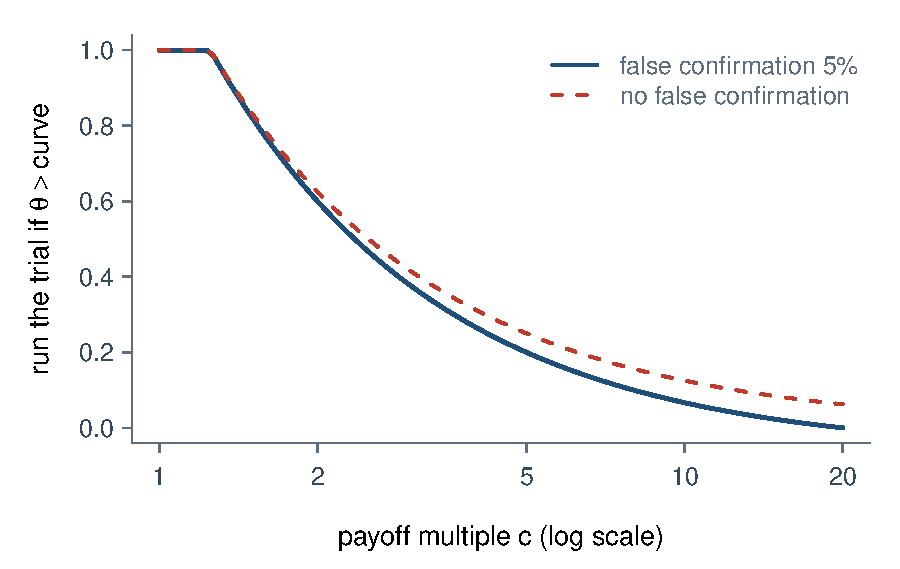
\includegraphics[width=0.62\linewidth]{ex02_decision.pdf}\end{center}
Without false confirmations ($\alpha=0$) the rule is simply $0.8\,c\,\theta>1$, i.e.\ $\theta>\frac{1.25}{c}$ (dashed curve).

\begin{answer}
Run the trial iff $c\{0.8\theta+0.05(1-\theta)\}>1$, i.e.\ $\theta>\frac{1/c-0.05}{0.75}$. It is never worth it if $c\le1.25$ (even a certainly-better drug is confirmed only 80\% of the time), and always worth it if $c\ge20$; e.g.\ with $c=2$ run it when $\theta>0.6$.
\end{answer}

\begin{takeaway}
Decision theory turns ``how sure are we?'' ($\theta$) and ``how much is at stake?'' ($c$) into a single, transparent rule.
\end{takeaway}

% ================================================================= Exercise 3
\exercise{9.3 --- Bias--variance tradeoff for a proportion}

\begin{problem}{3}
Assume $Y|\theta\sim\dist{Binomial}(n,\theta)$. Consider two estimators of $\theta$: the sample proportion $\hat\theta_1(Y)=Y/n$ and the posterior mean under the Jeffreys prior $\hat\theta_2(Y)=(Y+1/2)/(n+1)$.
\begin{enumerate}[(a)]
\item Compute the bias, variance and MSE for each estimator, and comment on the bias-variance tradeoff.
\item In terms of $n$ and the true value $\theta_0$, when is $\hat\theta_2(Y)$ preferred?
\end{enumerate}
\end{problem}

\begin{restate}
Compare the plain proportion with the slightly shrunken Jeffreys estimate in repeated samples.
\end{restate}

\begin{recall}
$\E(Y)=n\theta_0$, $\V(Y)=n\theta_0(1-\theta_0)$. For $\hat\theta=aY+b$: $\E\hat\theta=an\theta_0+b$, $\V\hat\theta=a^2n\theta_0(1-\theta_0)$.
\end{recall}

\begin{keyidea}
$\hat\theta_2=\frac{n}{n+1}\cdot\frac Yn+\frac1{n+1}\cdot\frac12$: a weighted average of $Y/n$ and $\frac12$ --- shrinkage toward $\frac12$ trades a little bias for less variance.
\end{keyidea}

\solution
\step{(a) $\hat\theta_1=Y/n$.} Bias $0$; variance $\frac{\theta_0(1-\theta_0)}{n}$; MSE $=\frac{\theta_0(1-\theta_0)}{n}$.
\step{(a) $\hat\theta_2=\frac{Y+1/2}{n+1}$.}
\[
\text{bias}=\frac{n\theta_0+\frac12}{n+1}-\theta_0=\frac{\frac12-\theta_0}{n+1},\qquad
\V=\frac{n\theta_0(1-\theta_0)}{(n+1)^2},\qquad
\text{MSE}=\frac{n\theta_0(1-\theta_0)+(\frac12-\theta_0)^2}{(n+1)^2}.
\]
Comment: $\hat\theta_2$ is biased toward $\frac12$, but its variance is smaller by the factor $\big(\frac{n}{n+1}\big)^2$. Both bias and the variance gap vanish as $n\to\infty$.
\step{(b) When does $\hat\theta_2$ win?} Write $v=\theta_0(1-\theta_0)$ and note $(\frac12-\theta_0)^2=\frac14-v$. Then $\text{MSE}_2<\text{MSE}_1$ iff
\[
n\big(nv+\tfrac14-v\big)<(n+1)^2v\iff\tfrac n4<(3n+1)v\iff\theta_0(1-\theta_0)>\frac{n}{12n+4}.
\]
\why{Multiply both MSEs by $n(n+1)^2$, expand $(n+1)^2v=n^2v+2nv+v$, and collect the $v$ terms.}
The bound increases to $\frac1{12}$ as $n\to\infty$, so $\hat\theta_2$ is better for $\theta_0$ in about $(0.09,\ 0.91)$: $n=5$: $(0.085,0.915)$; $n=20$: $(0.090,0.910)$; $n=100$: $(0.091,0.909)$.
\begin{center}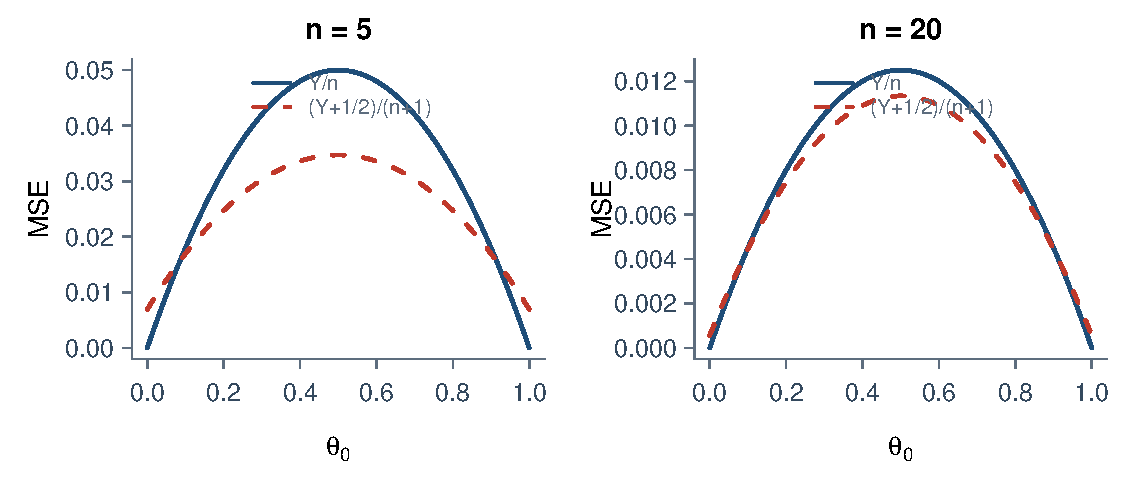
\includegraphics[width=0.95\linewidth]{ex03_mse.pdf}\end{center}

\begin{answer}
(a) $\hat\theta_1$: bias 0, MSE $\theta_0(1-\theta_0)/n$. $\hat\theta_2$: bias $\frac{1/2-\theta_0}{n+1}$, variance $\frac{n\theta_0(1-\theta_0)}{(n+1)^2}$, MSE $\frac{n\theta_0(1-\theta_0)+(1/2-\theta_0)^2}{(n+1)^2}$. (b) $\hat\theta_2$ has smaller MSE iff $\theta_0(1-\theta_0)>\frac{n}{12n+4}$, i.e.\ unless $\theta_0$ is within about 0.09 of 0 or 1.
\end{answer}

\begin{takeaway}
Unbiasedness is not optimality: a small, well-placed bias usually lowers the MSE.
\end{takeaway}

% ================================================================= Exercise 4
\exercise{9.4 --- Posterior mean vs.\ posterior mode for a variance}

\begin{problem}{4}
Assume $Y_1,\dots,Y_n|\sigma^2\iid\dist{Normal}(0,\sigma^2)$ and $\sigma^2\sim\dist{InvGamma}(a,b)$.
\begin{enumerate}[(a)]
\item Give an expression for two estimators of $\sigma^2$: the posterior mean and the posterior mode.
\item Plot the posterior density functions, and then give the two estimators for a sample with $n=10$ and $\sum_{i=1}^nY_i^2=200$ and $a=b=0.001$.
\item Argue that both estimators are consistent (i.e., their MSE goes to zero as $n$ increases) for any $a$ and $b$.
\end{enumerate}
\end{problem}

\begin{restate}
Two Bayesian point estimates of a normal variance: derive them, compute them for a sample, and show they both converge to the truth.
\end{restate}

\begin{recall}
$\sigma^2\mid\mathbf Y\sim\dist{InvGamma}(A,B)$ with $A=a+\frac n2$, $B=b+\frac12\sum Y_i^2$ (Exercise 2.8). $\dist{InvGamma}(A,B)$: mean $\frac{B}{A-1}$ ($A>1$), mode $\frac{B}{A+1}$. $\sum Y_i^2\sim\sigma^2\chi^2_n$ (mean $n\sigma^2$, variance $2n\sigma^4$).
\end{recall}

\begin{keyidea}
Both estimators are ``$\sum Y_i^2/2$ divided by roughly $n/2$'', so both behave like the MLE $\frac1n\sum Y_i^2$ for large $n$.
\end{keyidea}

\solution
\step{(a) Formulas.}
\[
\hat\sigma^2_{\text{mean}}=\frac{b+\frac12\sum Y_i^2}{a+\frac n2-1},\qquad\hat\sigma^2_{\text{mode}}=\frac{b+\frac12\sum Y_i^2}{a+\frac n2+1}.
\]
\why{The mode of $x^{-A-1}e^{-B/x}$: set the derivative of $-(A+1)\log x-B/x$ to zero: $-\frac{A+1}{x}+\frac B{x^2}=0\Rightarrow x=\frac B{A+1}$.}
\step{(b) Numbers.} $A=0.001+5=5.001$, $B=0.001+100=100.001$:
\[
\hat\sigma^2_{\text{mean}}=\frac{100.001}{4.001}=\mathbf{24.99},\qquad\hat\sigma^2_{\text{mode}}=\frac{100.001}{6.001}=\mathbf{16.66}\qquad(\text{MLE }200/10=20).
\]
\begin{center}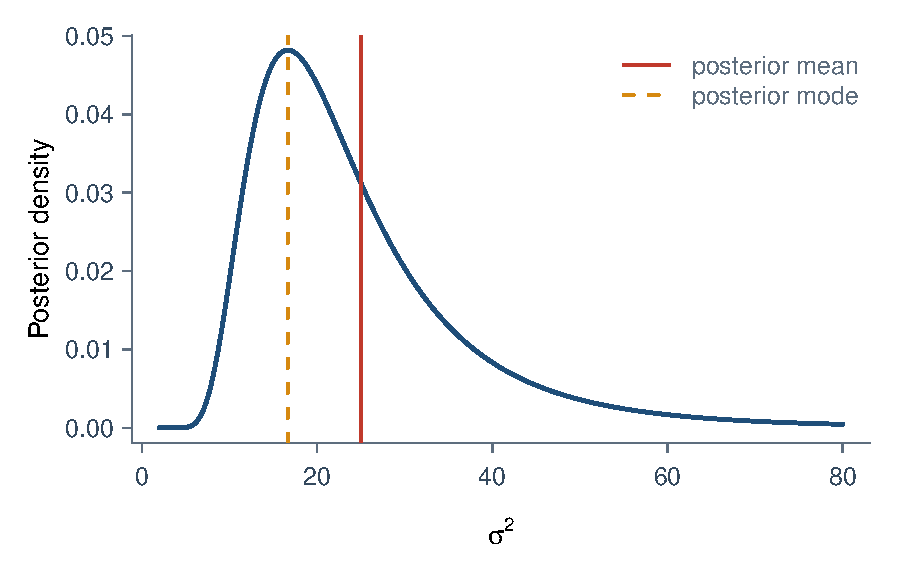
\includegraphics[width=0.62\linewidth]{ex04_posterior.pdf}\end{center}
The posterior is right-skewed, so the mean lies above the mode.
\step{(c) Consistency.} Write $\hat\sigma^2=\frac{b+S/2}{a+n/2+k}$ with $k=-1$ (mean) or $+1$ (mode), $S=\sum Y_i^2$. Then
\[
\E\hat\sigma^2=\frac{b+n\sigma^2/2}{a+n/2+k}\to\sigma^2,\qquad\V\hat\sigma^2=\frac{2n\sigma^4/4}{(a+n/2+k)^2}=O\Big(\frac1n\Big)\to0,
\]
so $\text{MSE}=\text{bias}^2+\V\to0$ for any fixed $a,b$. With $\sigma^2=20$: MSE(mean) $=149.9,\ 8.5,\ 0.80$ and MSE(mode) $=66.7,\ 7.8,\ 0.80$ for $n=10,100,1000$.

\begin{answer}
(a) Mean $\frac{b+\sum Y_i^2/2}{a+n/2-1}$, mode $\frac{b+\sum Y_i^2/2}{a+n/2+1}$. (b) 24.99 and 16.66. (c) Both have bias $O(1/n)$ and variance $O(1/n)$, so their MSE $\to0$: both are consistent, whatever $a,b$.
\end{answer}

\begin{takeaway}
For small $n$ the choice of point estimate matters (mean 25 vs.\ mode 17); asymptotically it does not.
\end{takeaway}

% ================================================================= Exercise 5
\exercise{9.5 --- Frequentist coverage of Jeffreys credible intervals}

\begin{problem}{5}
Assume $Y|\theta\sim\dist{Binomial}(n,\theta)$ and $\theta\sim\dist{Beta}(1/2,1/2)$. Use a simulation study to compute the empirical coverage of the equal-tailed 95\% credible set for $n\in\{1,5,10,25\}$ and true value $\theta_0\in\{0.05,0.10,\dots,0.50\}$. Comment on the frequentist properties of the Bayesian credible set.
\end{problem}

\begin{restate}
In repeated samples, how often does the Jeffreys 95\% interval contain the true success probability?
\end{restate}

\begin{recall}
$\theta\mid Y\sim\dist{Beta}(Y+\frac12,\ n-Y+\frac12)$; equal-tailed interval: its 2.5\% and 97.5\% quantiles. Because $Y$ takes only $n+1$ values, coverage can be computed \emph{exactly}: $\sum_{y=0}^n\dist{Binomial}(y;n,\theta_0)\,\mathbb 1\{\theta_0\in\text{CI}(y)\}$.
\end{recall}

\begin{keyidea}
Exact computation is the limit of an infinitely long simulation; we also ran a 10{,}000-replicate simulation to check.
\end{keyidea}

\solution
\begin{center}
\small
\begin{tabular}{c|cccc}\toprule
$\theta_0$ & $n=1$ & $n=5$ & $n=10$ & $n=25$\\\midrule
0.05 & 0.950 & 0.977 & 0.988 & 0.966\\
0.10 & 0.900 & 0.991 & 0.987 & 0.895\\
0.15 & 1.000 & 0.973 & 0.950 & 0.957\\
0.20 & 1.000 & 0.942 & 0.967 & 0.955\\
0.25 & 1.000 & 0.984 & 0.924 & 0.938\\
0.30 & 1.000 & 0.969 & 0.924 & 0.949\\
0.35 & 1.000 & 0.946 & 0.961 & 0.942\\
0.40 & 1.000 & 0.912 & 0.941 & 0.936\\
0.45 & 1.000 & 0.931 & 0.949 & 0.957\\
0.50 & 1.000 & 0.937 & 0.979 & 0.957\\\midrule
average & 0.985 & 0.956 & 0.957 & 0.945\\\bottomrule
\end{tabular}
\end{center}
\begin{center}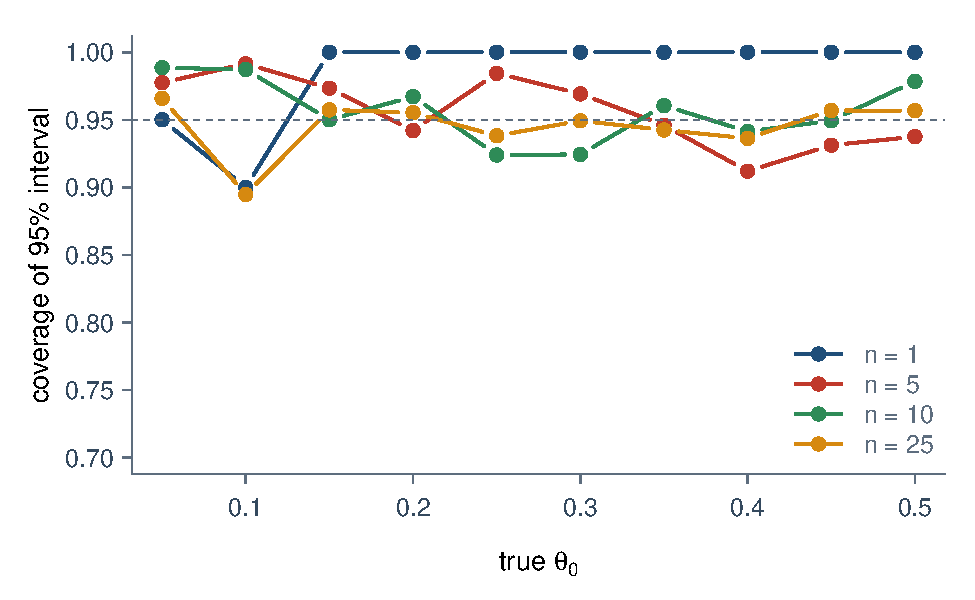
\includegraphics[width=0.7\linewidth]{ex05_coverage.pdf}\end{center}
The simulation agrees with the exact values to within 0.006.

\step{Comments.}
\begin{itemize}
\item On \emph{average} over $\theta_0$ the coverage is close to 95\% even for tiny $n$ --- the Jeffreys interval has good frequentist properties (it is known to beat the classical Wald interval).
\item For a \emph{given} $\theta_0$ the coverage jumps around (from 0.89 to 0.99 for $n=25$) because $Y$ is discrete: as $\theta_0$ moves, whole outcomes enter or leave the interval. No interval for a binomial proportion can have exactly 95\% coverage everywhere.
\item With $n=1$ the interval is very wide, so coverage is usually 100\% (but 90\% at $\theta_0=0.1$).
\end{itemize}

\begin{answer}
The Jeffreys equal-tailed interval has approximately nominal coverage on average (0.95--0.96 for $n\ge5$), with oscillations between about 0.89 and 0.99 due to the discreteness of $Y$; for $n=1$ it is conservative.
\end{answer}

\begin{takeaway}
A Bayesian interval with a sensible default prior is often an excellent \emph{frequentist} interval too.
\end{takeaway}

% ================================================================= Exercise 6
\exercise{9.6 --- A Bayesian re-analysis from a published estimate}

\begin{problem}{6}
A paper reports the results of a logistic regression analysis using maximum likelihood estimation. They estimate $\beta_1$ to be $\hat\beta_1=1.8$, with the 95\% confidence interval (0.42, 3.17). Further, the p-value for the test that $H_0:\beta_1=0$ versus $H_1:\beta_1\neq0$ is 0.01. Conduct a Bayesian analysis using only this information and asymptotic arguments.
\end{problem}

\begin{restate}
We only have a point estimate, an interval and a p-value. Turn them into an approximate likelihood and do a Bayesian analysis.
\end{restate}

\begin{recall}
Large-sample likelihood: $\hat\beta_1\mid\beta_1\approx\dist N(\beta_1,\ \text{SE}^2)$ (primer, point 3); a 95\% CI is $\hat\beta\pm1.96\,\text{SE}$. Normal prior $\dist N(0,\tau^2)$ $\Rightarrow$ posterior $\dist N\big(\frac{\hat\beta/\text{SE}^2}{1/\text{SE}^2+1/\tau^2},\ \frac1{1/\text{SE}^2+1/\tau^2}\big)$. Point-null BF: $\frac{\dist N(\hat\beta;0,\text{SE}^2+\tau^2)}{\dist N(\hat\beta;0,\text{SE}^2)}$ (as in equation 5.10).
\end{recall}

\begin{keyidea}
Recover the SE from the interval, check it against the p-value, then combine the normal ``likelihood'' with a few priors.
\end{keyidea}

\solution
\step{Step 1 --- the standard error.} $\text{SE}=\frac{3.17-0.42}{2\times1.96}=0.70$. Check: $z=1.8/0.70=2.57$, two-sided $p=0.010$ --- consistent with the reported $p=0.01$ (and the interval is symmetric about 1.8, as a Wald interval should be).
\step{Step 2 --- posteriors under several priors.}
\begin{center}
\small
\begin{tabular}{lccccc}\toprule
Prior on $\beta_1$ & posterior mean & 95\% CI & $\Prob(\beta_1>0)$ & mean odds ratio & BF($H_1$:$H_0$)\\\midrule
flat & 1.80 & (0.43, 3.17) & 0.995 & 7.7 & ---\\
$\dist N(0,2^2)$ & 1.60 & (0.31, 2.90) & 0.992 & 6.2 & 6.2\\
$\dist N(0,1^2)$ & 1.21 & (0.08, 2.33) & 0.982 & 3.9 & 5.2\\
$\dist N(0,0.5^2)$ (sceptical) & 0.61 & $(-0.19,\ 1.40)$ & 0.932 & 2.0 & 2.5\\\bottomrule
\end{tabular}
\end{center}
\begin{center}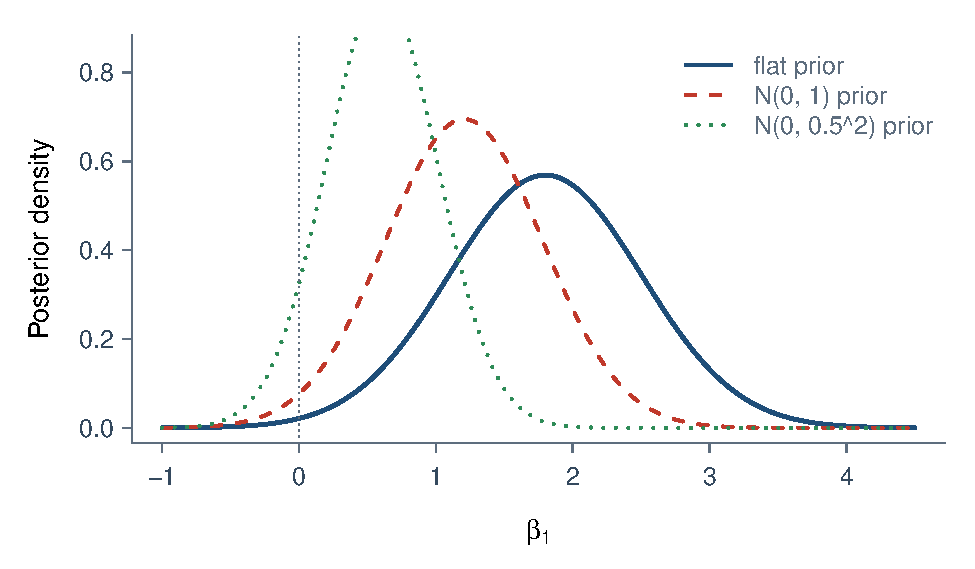
\includegraphics[width=0.7\linewidth]{ex06_posterior.pdf}\end{center}
\why{With a flat prior the posterior reproduces the confidence interval numerically, but now it may be read as ``95\% probability that $\beta_1$ lies in (0.43, 3.17)''. The mean odds ratio is $\E(e^{\beta_1})=e^{m+s^2/2}$ for a normal posterior.}

\begin{answer}
$\beta_1\mid\text{data}\approx\dist N(1.8,\ 0.70^2)$ under a flat prior: $\Prob(\beta_1>0)=0.995$, 95\% interval (0.43, 3.17). Reasonable sceptical priors shrink the estimate (e.g.\ to 1.21 with $\dist N(0,1)$) but keep $\Prob(\beta_1>0)\ge0.93$. The point-null Bayes factor is only 2.5--6.2 --- much weaker evidence than ``$p=0.01$'' suggests.
\end{answer}

\begin{takeaway}
A $p$-value of 0.01 corresponds to a Bayes factor of only about 3--6 against the point null: $p$-values overstate the evidence against $H_0$.
\end{takeaway}

% ================================================================= Exercise 7
\exercise{9.7 --- How many customers for a posterior SD of 0.01?}

\begin{problem}{7}
You are designing a study to estimate the success probability of a new marketing strategy. When the data have been collected, you will analyze them using the model $Y|\theta\sim\dist{Binomial}(n,\theta)$ and $\theta\sim\dist{Uniform}(0,1)$. Before collecting any data, you suspect (based on past studies) that $\theta\approx0.4$. Which value of $n$ should be used to ensure the posterior standard deviation will be approximately 0.01?
\end{problem}

\begin{restate}
Choose the sample size so that, after the study, we will know the success rate to within about $\pm0.01$ (one posterior SD).
\end{restate}

\begin{recall}
$\theta\mid Y\sim\dist{Beta}(Y+1,\ n-Y+1)$, whose variance is $\frac{ab}{(a+b)^2(a+b+1)}$ with $a+b=n+2$. If $Y\approx n\theta$ this is $\approx\frac{\theta(1-\theta)}{n+3}$.
\end{recall}

\begin{keyidea}
Plug in the guess $\theta=0.4$ and solve for $n$; then check by averaging the exact posterior SD over the possible outcomes $Y$.
\end{keyidea}

\solution
\step{Approximation.} $\sqrt{\frac{0.4\times0.6}{n+3}}=0.01\iff n+3=\frac{0.24}{0.0001}=2400\iff n=2397$.
\step{Exact check.} Averaging the exact Beta posterior SD over $Y\sim\dist{Binomial}(2397,0.4)$ gives 0.01000, and 2397 is the smallest $n$ for which it is $\le0.01$.
\step{Sensitivity to the guess.} If $\theta$ were 0.3 the SD at $n=2397$ would be 0.0094; if 0.5, 0.0102 --- the worst case $\theta=0.5$ would need $n=2497$.

\begin{answer}
$n\approx2{,}400$ (precisely $n=2397$ under $\theta\approx0.4$; use $n\approx2{,}500$ to be safe for any $\theta$).
\end{answer}

\begin{takeaway}
Posterior precision grows like $\sqrt n$: halving the posterior SD needs four times as many observations.
\end{takeaway}

% ================================================================= Exercise 8
\exercise{9.8 --- Exponential families, conjugacy and unbiasedness}

\begin{problem}{8}
Suppose $Y_1,\dots,Y_n\iid f(y|\eta)$ where $f$ is the canonical exponential family
\[
f(y|\eta)\propto\exp\{y\eta-\psi(\eta)\}
\]
for some known function $\psi$. We are interested in estimating the parameter $\theta=E(Y_i|\eta)=d\psi(\eta)/d\eta$.
\begin{enumerate}[(a)]
\item Show that the Gaussian density with variance fixed at one and the Poisson density can be written in this form.
\item Obtain the maximum likelihood estimator of $\theta$. Is it unbiased for $\theta$?
\item Find a class of conjugate priors for $\eta$.
\item Obtain the Bayes estimator of $\theta$ using a conjugate prior and squared error loss.
\item Is there any (proper) conjugate prior for which the Bayes estimator that you obtained in (d) is unbiased? Justify your answer.
\end{enumerate}
\end{problem}

\begin{restate}
For the whole exponential family at once: write two familiar models in canonical form, find the MLE and the conjugate prior, and show that the Bayes estimator can never be unbiased under a proper conjugate prior.
\end{restate}

\begin{recall}
Primer, point 4: $\E(Y\mid\eta)=\psi'(\eta)$. \textbf{Diaconis--Ylvisaker (1979)}: for the conjugate prior below, the prior mean of $\psi'(\eta)$ is $y_0$, and the posterior mean of $\psi'(\eta)$ is a weighted average of $y_0$ and $\bar Y$.
\end{recall}

\begin{keyidea}
The conjugate posterior mean is $\frac{n_0y_0+n\bar Y}{n_0+n}$: it always puts weight $\frac{n_0}{n_0+n}>0$ on the prior guess $y_0$, which creates bias.
\end{keyidea}

\solution
\step{(a) Gaussian, variance 1.} $f(y\mid\mu)\propto\exp\{-\frac{(y-\mu)^2}2\}=\exp\{y\mu-\frac{\mu^2}{2}\}\,e^{-y^2/2}$: $\eta=\mu$, $\psi(\eta)=\frac{\eta^2}2$ (the factor $e^{-y^2/2}$ does not involve $\eta$). Check: $\psi'(\eta)=\eta=\mu=\E Y$. \checkmark

\textbf{Poisson.} $f(y\mid\lambda)=\frac{e^{-\lambda}\lambda^y}{y!}=\exp\{y\log\lambda-\lambda\}\frac1{y!}$: $\eta=\log\lambda$, $\psi(\eta)=e^\eta$. Check: $\psi'(\eta)=e^\eta=\lambda=\E Y$. \checkmark
\step{(b) MLE.} $\ell(\eta)=\eta\sum Y_i-n\psi(\eta)$, so $\ell'(\eta)=\sum Y_i-n\psi'(\eta)=0\Rightarrow\psi'(\hat\eta)=\bar Y$. By invariance, $\hat\theta_{\text{MLE}}=\psi'(\hat\eta)=\bar Y$, which is unbiased: $\E\bar Y=\theta$.
\step{(c) Conjugate prior.} Take a prior with the same shape as the likelihood in $\eta$:
\[
\pi(\eta\mid n_0,y_0)\propto\exp\{n_0y_0\eta-n_0\psi(\eta)\},\qquad n_0>0,
\]
(like $n_0$ prior observations with mean $y_0$). Then
\[
p(\eta\mid\mathbf Y)\propto\exp\{(n_0y_0+n\bar Y)\eta-(n_0+n)\psi(\eta)\}:
\]
the same family with $n_0\to n_0+n$ and $y_0\to\frac{n_0y_0+n\bar Y}{n_0+n}$.
\step{(d) Bayes estimator under squared-error loss} = posterior mean of $\theta=\psi'(\eta)$. For this family (Diaconis--Ylvisaker) $\E\{\psi'(\eta)\}=y_0$ under the prior $\pi(\cdot\mid n_0,y_0)$; applying this to the posterior,
\[
\hat\theta_{\text{Bayes}}=\E\{\psi'(\eta)\mid\mathbf Y\}=\frac{n_0y_0+n\bar Y}{n_0+n}.
\]
\why{The prior result follows by integrating $\frac{\dd}{\dd\eta}\pi(\eta)=n_0\{y_0-\psi'(\eta)\}\pi(\eta)$ over $\eta$: the left side integrates to 0 (the density vanishes at the ends of its range), so $\E\{\psi'(\eta)\}=y_0$.}
For example, normal: $\frac{n_0y_0+n\bar Y}{n_0+n}$ is the normal--normal posterior mean; Poisson: $\lambda\sim\dist{Gamma}(n_0y_0,n_0)$ gives $\frac{n_0y_0+\sum Y_i}{n_0+n}$.
\step{(e) Can it be unbiased?}
\[
\E\big(\hat\theta_{\text{Bayes}}\mid\theta\big)=\frac{n_0y_0+n\theta}{n_0+n}=\theta\iff n_0(y_0-\theta)=0.
\]
For this to hold for \emph{every} $\theta$ we need $n_0=0$, but then $\pi(\eta)\propto1$, which is improper. So \textbf{no proper conjugate prior gives an unbiased Bayes estimator} (except trivially at the single point $\theta=y_0$).

\begin{answer}
(a) Normal: $\eta=\mu$, $\psi=\eta^2/2$; Poisson: $\eta=\log\lambda$, $\psi=e^\eta$. (b) $\hat\theta=\bar Y$, unbiased. (c) $\pi(\eta)\propto\exp\{n_0y_0\eta-n_0\psi(\eta)\}$. (d) $\hat\theta_{\text{Bayes}}=\frac{n_0y_0+n\bar Y}{n_0+n}$. (e) No: unbiasedness for all $\theta$ requires $n_0=0$, an improper prior.
\end{answer}

\begin{takeaway}
This is a special case of a general theorem: under squared-error loss, a Bayes estimator with a proper prior is never unbiased (unless it estimates $\theta$ perfectly). Bayesian estimators deliberately accept bias for lower MSE (Exercise 3).
\end{takeaway}

\end{document}
